%DAQ_Measuremnt_V
Let's review what we learned last week. In physics equipment, we try to
measure voltages. If your data is not a voltage, we try to convert it into a
voltage. Already we converted current into a voltage (using a shunt
resistor). But what is a voltage? We said last week that it is a measure of
electrical potential energy. It is also likely that you know the word
\textquotedblleft voltage\textquotedblright\ because we live in a world that
has electricity everywhere. You probably know that your house or apartment
has wires in the walls that carry \textquotedblleft 110
Volts.\textquotedblright\ And you probably realize that \textquotedblleft
voltage\textquotedblright\ is a measure of how much energy there is in the
wires.

Soon your PH220 class will explain that \textquotedblleft
voltage\textquotedblright\ is proportional to the electrical potential
energy difference. But for us, now, we just need to know that we are
measuring something proportional to energy and we need to learn how to
measure it.

Because voltage is proportional to a \emph{difference} in electrical
potential energy, a voltage measurement really is a combination of two
measurements. Think of gravitational potential energy. If we ask for the
potential energy difference as Super Guy jumps from the bottom of a building
to the top \begin{figure}[h!]
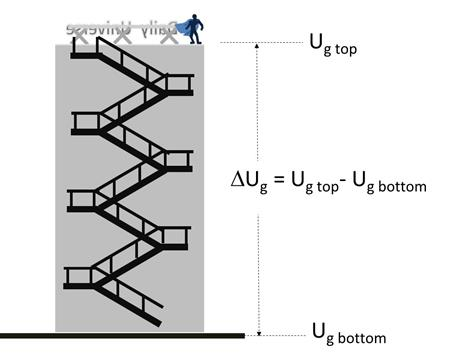
\includegraphics[width=3.781in,height=3.0191in]{PH4CAU1I}
\end{figure}we need two measurements, one at
the bottom and one at the top. Then 
\begin{equation*}
\Delta U_{g}=U_{g_{top}}-U_{g_{bottom}}
\end{equation*}

We will do something very similar in measuring voltages. We will measure the
potential energy at two places. For example, suppose we have an electric
circuit as shown in the next figure. \begin{figure}[h!]
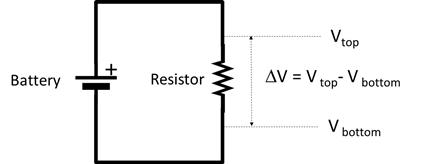
\includegraphics[width=3.5466in,height=1.3932in]{PH4CAU1J}
\end{figure}The circuit is very simple, just
a battery and a resistor. You have experience with batteries, and resistors
now. A resistor is just a piece of material that has lots of electrical
friction, or \textquotedblleft resistance\textquotedblright\ that makes it
hard for electrons to go through it. If we want to measure the voltage
across the resistor, we have to measure on the top and bottom of the
resistor. That will give us a measurement proportional to the potential
energy difference from one side to the other of the resistor.

Most meters that measure voltage have two \textquotedblleft
probes\textquotedblright\ and do the difference calculation internally.
These meters are called \emph{voltmeters} and we used them last week. \begin{figure}[h!]
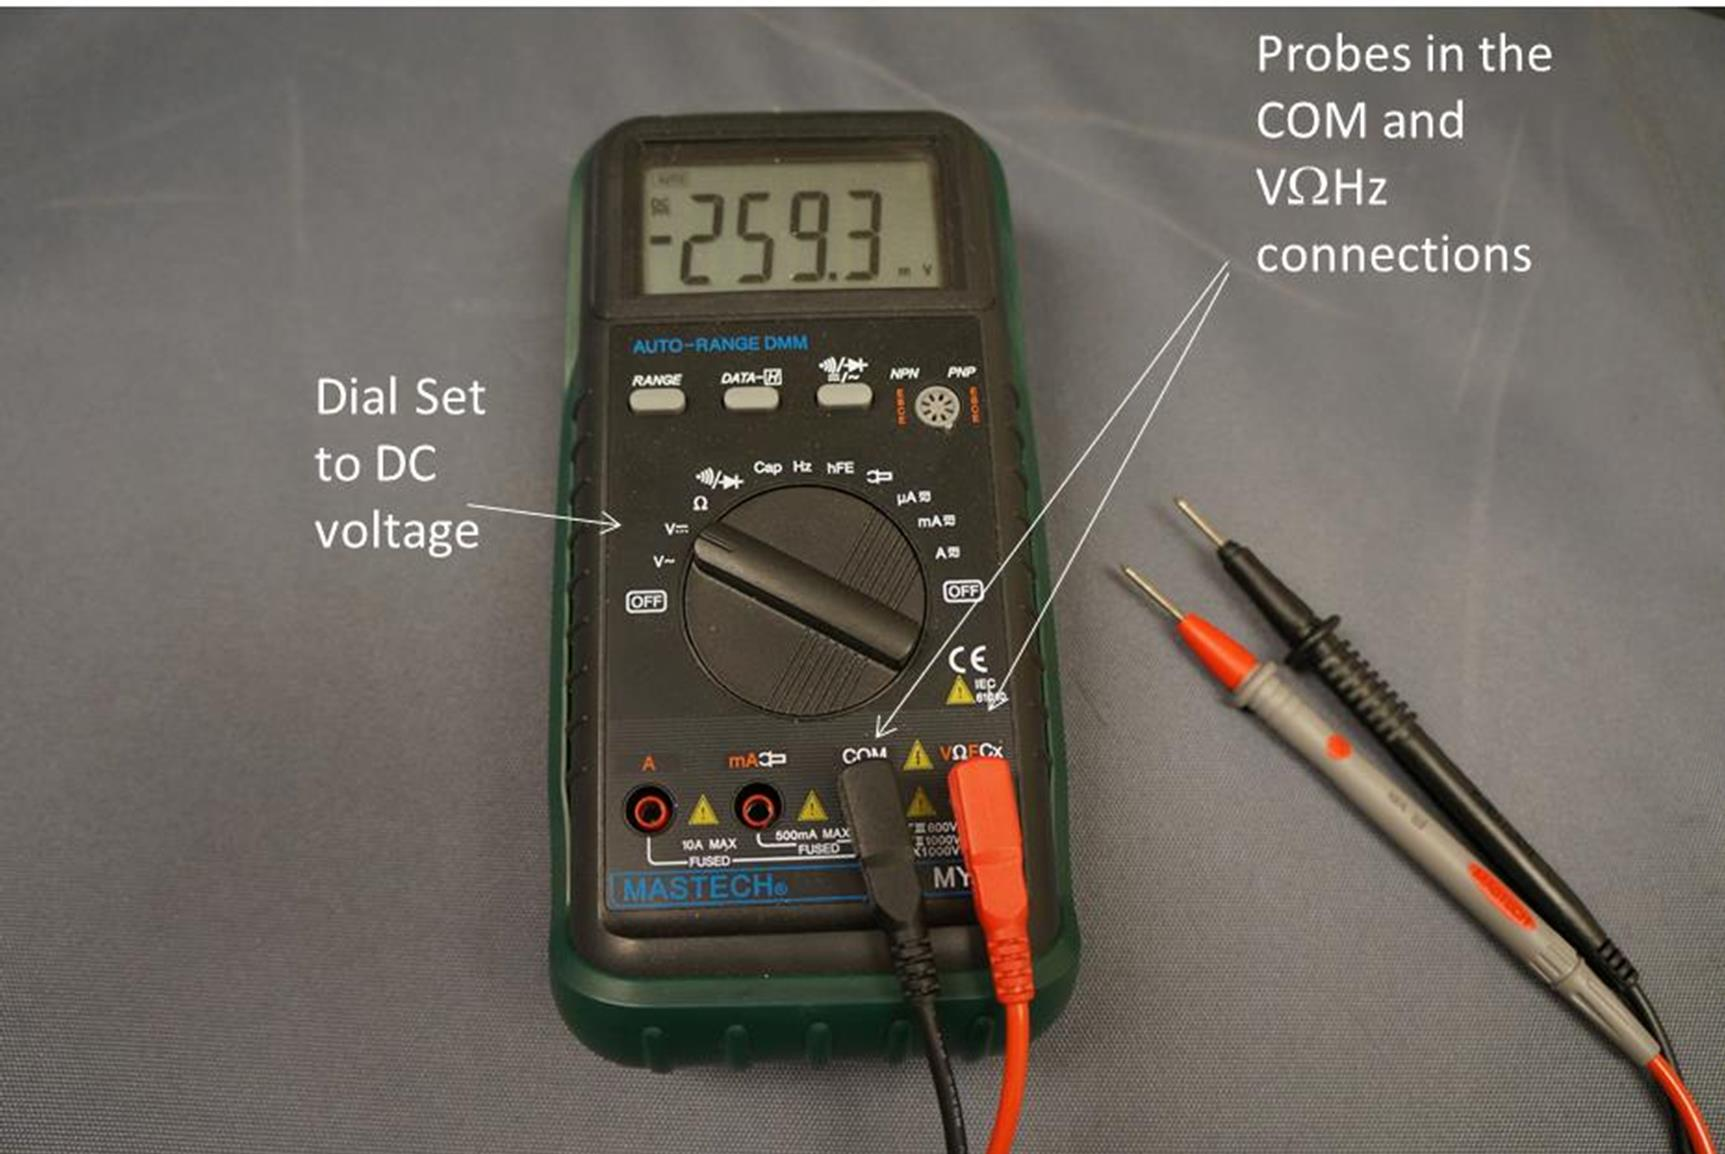
\includegraphics[width=2.9199in,height=1.962in]{PH4CAU1K}
\end{figure}%
In today's world, voltmeters are usually just one part of a device that can
measure many things. We call these devices multimeters. To measure voltage
we will set the multimeter on the DC Voltage setting. Notice the two probe
wires in the figure. We need two probes to make the two measurements and the
device does the subtraction for us.

We learned to use a sand-alone voltmeter in the last lab. But we also need
to read in voltages in a way that the data shows up on our computer. To get
the data into our computer we will use a different set of pins on our
Arduino board. They are called \emph{analog} pins.

Even before we begin, we need a warning. We absolutely must not wire up the
analog pins on our Arduino backwards! This can (and probably will) destroy
the pin circuitry inside our Arduino. So we will need to be careful in
wiring for this part of our lab. Where this could be a problem a warning
sign will appear in the text, just to remind you to be careful! \begin{figure}[h!]
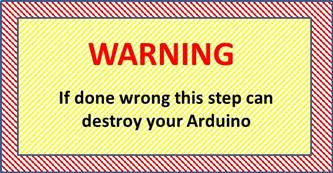
\includegraphics[width=2.8089in,height=1.4684in]{PH4CAU1L}
\end{figure}%
You may see quite a few of these in this lab.

\section{Building a voltmeter}

Our Arduino has what we call and Analog to Digital converter (ADC). That is,
it takes analog voltage signals that could have any value, and it maps them
into a set of discrete values and sort of rounds to the nearest whole
discrete value.

The word \textquotedblleft analog\textquotedblright\ might not be familiar.
Think of our power supply. It has a knob that adjusts the voltage. The knob
can produce any voltage from $0$ to about $30\unit{V}$. This is an analog
signal. The voltage can take on any value in a range. So we represent an
analog signal with real numbers and we might have a voltage of exactly 
\begin{equation*}
4.3276854325532573457\unit{V}
\end{equation*}%
and this would be perfectly valid for an analog signal.

A battery, on the other hand, is not this way. It has a fixed voltage, say, $%
1.5\unit{V}$ like the D-Cell batteries that we used in our last lab. Two
D-Cell batteries could be used together to make $3\unit{V}.$ But you can't
use D-Cell batteries to get $2.25\unit{V}.$ The batteries come in discrete
units.

Our Arduino analog pin is designed to measure voltages in the range $0$ to $5%
\unit{V}.$ Don't set your power supply to more than $5\unit{V}!$ But there
is more to the ADC than just a voltage range. The Arduino chops the voltage
range into 1024 discrete voltage divisions. Each division is then%
\begin{equation*}
\Delta v_{\min }=\frac{5\unit{V}}{1024}=4.\,\allowbreak 9\unit{mV}
\end{equation*}%
\begin{figure}[h!]
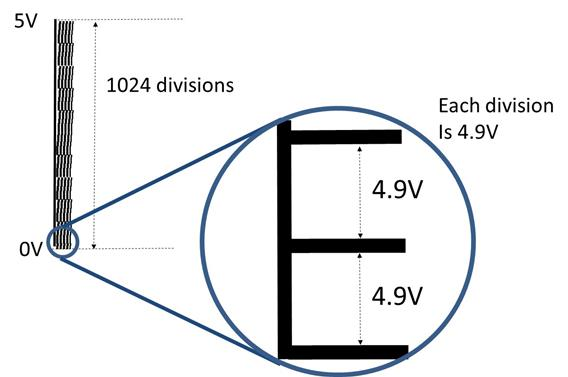
\includegraphics[width=2.3618in,height=1.5714in]{PH4CAU1M}
\end{figure} This means that changes in
voltage that are less than $4.9\unit{mV}$ won't be seen, since it takes a
whole $4.9\unit{mV}$ to get a different division. So if we give our Arduino $%
8\unit{mV}$ this is not enough to fill the second $4.9\unit{mV}$ division,
so our Arduino would still read only $4.9\unit{mV}.$ If we gave it $11\unit{%
mV}$ it would then read $9.8\unit{mV}$ because $9.8\unit{mV}=2\times 4.9%
\unit{mV}$ and $9.8$ is the closest whole unit of $4.9\unit{mV}.$\begin{figure}[h!]
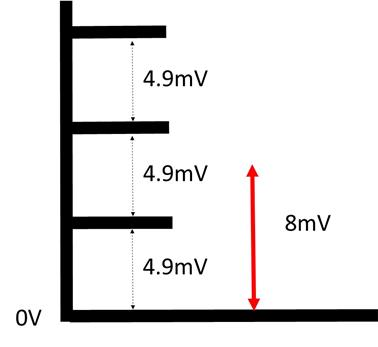
\includegraphics[width=3.1868in,height=2.9265in]{PH4CAU1N}
\end{figure}%
This is called \textquotedblleft discretization\textquotedblright\ or more
commonly \textquotedblleft digitization\textquotedblright\ or even
\textquotedblleft \emph{quantization.\textquotedblright\ } We have taken a
signal that might have any value between $0$ to $5\unit{V}$ and we output a
signal that will be rounded to the nearest $n\times 4.9\unit{mV}.$

As a second example, $3.793\unit{V}$ would be reported as $\allowbreak
3.792\,\allowbreak 6\unit{V}$ since 
\begin{equation*}
\frac{3.793\unit{V}}{4.9\unit{mV}}=774.\,\allowbreak 08
\end{equation*}%
but we need even units of $\Delta v_{\min },$ so the $0.8$ would be dropped
by the A2D converter giving 
\begin{equation*}
774\times 4.9\unit{mV}=\allowbreak 3.792\,\allowbreak 6\unit{V}
\end{equation*}%
and our first voltage from our power supply, $4.3276854325532573457\unit{V}$
would be reported as $4.\,\allowbreak 326\,7\unit{V}$ (make sure you can see
how we got this result!).

This means that we can be off in our voltage measurements as much as $4.9%
\unit{mV}$! In dividing up our voltage range into $1024$ pieces we have
introduced some error, but we have divided our $0$ to $5\unit{V}$ into
numeric values that we can use in our computer, so it is worth the cost of
some error.

The amount of error depends on how many different values the ADC converter
has. Since breaking an analog signal into discrete values is called \emph{%
quantization, }we call this source of error \emph{quantization error.} It is
the source of much of the error we see in electronic measuring devices. We
could say that our new voltmeter has an uncertainty of at least the voltage
resolution%
\begin{equation*}
\delta V_{signal}=\Delta V_{\min }=4.\,\allowbreak 9\unit{mV}
\end{equation*}%
but of course it could be larger if there are other sources of error.

The ADC sends the measured value through our USB\ cable to our computer's
serial port. But it doesn't send it in units of volts. It sends it in ADC
units. If we have a signal voltage of $9.8\unit{mV}$ we don't get out $9.8,$
we get $2$ because $9.8\unit{mV}=2\Delta V_{\min }.$ The ADC units are the
number of $\Delta V_{\min }$ sized units that are in our signal voltage. To
get back to voltage units, we need to multiply by $\Delta V_{\min }.$ In our
code we will do this before reporting the value.

Of course we would like to see the voltage that we measure. There is a
simple way to do this. The voltage values we calculate can be sent to our
computer through the serial cable. We will need an Arduino sketch with some
additional setup and some additional loop commands. One of these commands
will turn our ADC\ units into volts.

Before we look at the entire sketch, let me introduce the new commands that
we will need. To get the Arduino to communicate with the computer we use the
command 
\begin{equation*}
\begin{tabular}{l}
\ Serial.begin();%
\end{tabular}%
\end{equation*}%
and in the loop function we use the command\ 
\begin{equation*}
\begin{tabular}{l}
\ Serial.print();%
\end{tabular}%
\end{equation*}

We also need to know that computers make a distinction between integer and
real numbers. Our voltages will be real numbers, so we need to tell the
Arduino that we want a real number. The command for this is the word
\textquotedblleft float.\textquotedblright\ For example,%
\begin{equation*}
\begin{tabular}{l}
\ float\ delta\_v\_min=0.0049;%
\end{tabular}%
\end{equation*}%
defines a variable named \textquotedblleft delta\_v\_min\textquotedblright\
and sets it to the value $0.0049.$ If we want an integer number we use the
word \textquotedblleft int.\textquotedblright\ For example%
\begin{equation*}
\begin{tabular}{l}
\ int\ value\ =\ 0;%
\end{tabular}%
\end{equation*}%
defines a variable named \textquotedblleft value\textquotedblright\ and sets
it equal to $0.$ All this is a little like listing your variables back in
PH121. Only here if you don't do it, it doesn't just cost you points, it
confuses the Arduino software and the Arduino software will give you an
error.

We also need special commands to read our Arduino analog pins. The special
Arduino command 
\begin{equation*}
\begin{tabular}{l}
analogRead()%
\end{tabular}%
\end{equation*}%
will do this.

The whole Arduino sketch might look like this:
\begin{lstlisting}[language=Arduino]
/////////////////////////////////////////////////////////
// very simple voltmeter
// will measure 0 to 5V only!
// Voltages outside 0 to 5V will destroy your Arduino!!!
// Don't wire this backwards!
/////////////////////////////////////////////////////////
// define a variable that tells which analog pin we will 
//   use
int AI0 = 0;    //AI0 stands for analog input zero
// define a variable that holds our Delta_v_min
float delta_v_min=0.0049;   // volts per A2D unit
// define a variable for our A2D version of our signal
int ADC_value = 0;
// define a variable for our voltage version of our signal
float voltage = 0.0;
 
/////////////////////////////////////////////////////////
void setup() {
  // put your setup code here, to run once when your
  // Arduino starts up:
  //
  // Initiate Serial Communication, so we can see the
  // voltage on our computer
  Serial.begin(9600);    //9600 baud rate
}
 
/////////////////////////////////////////////////////////
void loop() {
  // Read in the voltage in A2D units form the serial port
  //   remember that AI0 is the pin number to read from
  ADC_value = analogRead(AI0); 
  // Let's print out our A2D version of our signal
  Serial.print(" A2D ");
  Serial.print(ADC_value); 
  // Now convert to voltage units using delta_v_min
  voltage = ADC_value * delta_v_min;
  // And print out our voltage version of our signal
  Serial.print(" voltage ");
  // Print the voltage with 4 significant figures)
  Serial.println(voltage, 4);  
}
/////////////////////////////////////////////////////////
/////////////////////////////////////////////////////////
 \end{lstlisting}

\ 

Make sure you understand every line of this code. Write it in the Arduino
IDE and run it to help see what the lines do. Lines that begin with two
slashes, \textquotedblleft //,\textquotedblright\ are comments. The Arduino
will ignore these lines. But you shouldn't! The comments tell you, the
programmer, what the code is doing. I will ask you in lab to input comments
for every line. If there is any part of this sketch that is mysterious, work
with your group to resolve the mystery and if it is still mysterious, call
your instructor over to discuss the sketch with you.

\subsection{Wiring the simple voltmeter}

\begin{figure}[h!]
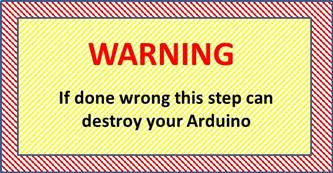
\includegraphics[width=1.8507in,height=0.9677in]{PH4CAU1O}
\end{figure}You knew that was coming, didn't
you! We must be very careful to wire our Arduino correctly. Our Arduino can
measure $0$ to $5\unit{V}.$ But if we switch the $5\unit{V}$ and the $0\unit{%
V}$ by plugging them into the wrong pin, our Arduino will be damaged and
will never work the same way again (probably won't work at all!). So wire


\section{Building a New Instrument}

We said before that physicists like to change any measurement they can into
a voltage measurement. That is because we have devices like our Arduino
boards that measure voltage. We build new instruments by finding ways to
turn the measurement that we want to make into a voltage.

In order to build a new instrument, we need to understand the quantity that
we really want to measure. We will need to understand the physics of the
quantity to make a good new instrument design. Let's take an example.
Suppose we wish to measure current, but suppose we don't have a current
setting on our Arduino (because we don't). Could we still make a current
measurement?

The secret of instrument design is to understand the physics of the
measurement we want to make (current) and then see if we can turn that
measurement into a voltage.

\subsection{Start with the Physics:}

Let's keep thinking of current like water in a hose. Will there be any
friction associated with the water traveling through the hose? Of course
there will! We usually call friction in fluids \emph{viscosity}. But it is a
form of friction, and we can use our PH121 intuition about friction to see
how it would work. Think of having two hoses, one twice as long as the
other. Which would you expect to have more friction? \begin{figure}[h!]
	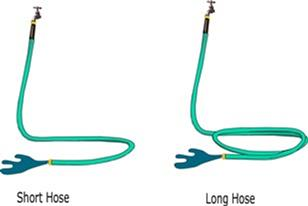
\includegraphics[width=2.6033in,height=%
	1.7474in]{PH4CAU0Z}
\end{figure}

Our friction experience says that the longer the path, the more the
friction. The current has longer to interact with the hose, so it
experiences more friction. Electrical currents are like this. Longer wires
give more friction.

George Simon Ohm noticed that with long metal wires, there seemed to be a
linear relationship between the potential difference (voltage), the current,
and the length of the wire. The longer the wire, the less the current. His
work was confirmed and expanded on by others, who found that not only length
mattered, but also the diameter of the wire mattered. The relationship is
now expressed as%
\begin{equation*}
\Delta V=IR
\end{equation*}%
$\Delta V$ is our old friend, voltage, and we know $I$ is the symbol for
current, and $R$ is the slope of the $\Delta V$ vs. $I$ curve. The
experiments showed this constant $R$ depended on the material. It is like
our viscosity in hoses. It is the friction. The more the friction, the
harder it is to get the current through the wire. But like we don't call
viscosity \textquotedblleft friction,\textquotedblright\ we also don't use
the word \textquotedblleft friction\textquotedblright\ for this
friction-like term. We call it \emph{resistance.} We could solve for this
resistance 
\begin{equation*}
R=\frac{\Delta V}{I}
\end{equation*}%
or we could plot $\Delta V$ vs. $I$ and the slope of this line would be the
resistance.\begin{figure}[h!]
	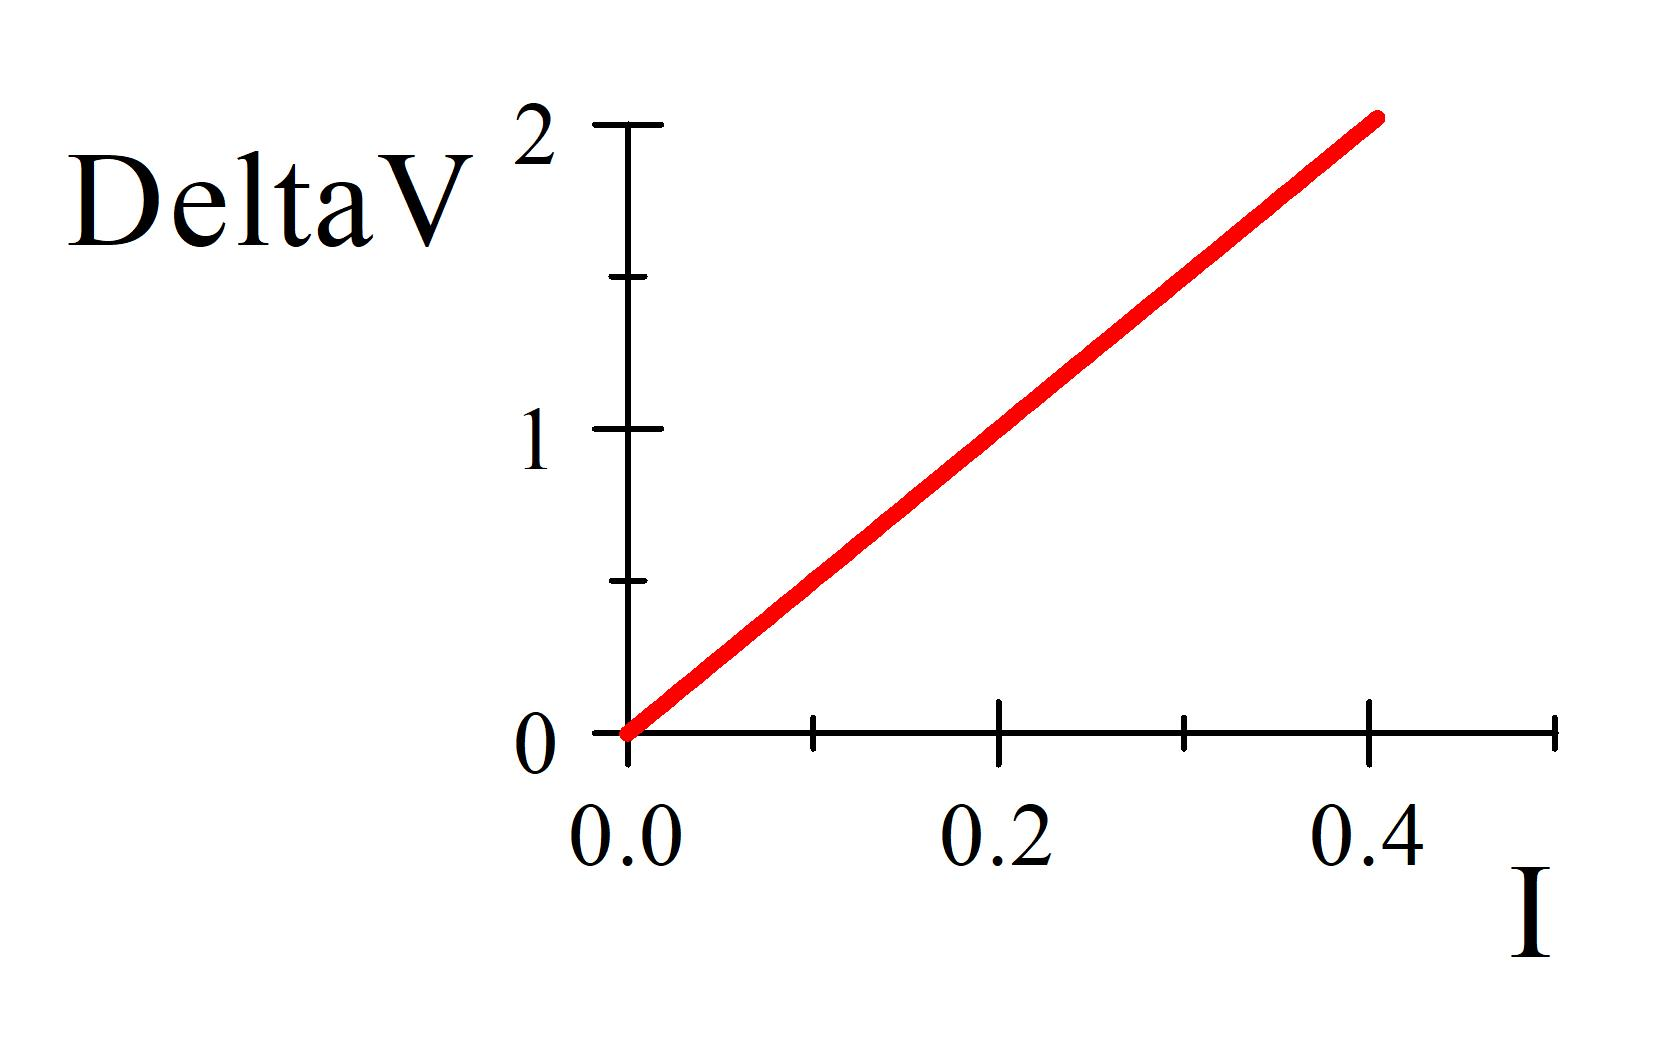
\includegraphics[width=1.9899in,height=1.3214in]{PH4CAU10}
\end{figure}Either way, this relationship
tells us that it takes more potential energy to get the same current if
there is more resistance.

This is called \emph{Ohm's law.} The relationship holds well for metals and
many materials, but, like Hook's law, this \textquotedblleft
law\textquotedblright\ does not always hold. Devices that do provide a
constant resistance coefficient, $R,$ are called \emph{resisters. }We will
use this symbol

\begin{figure}[h!]
	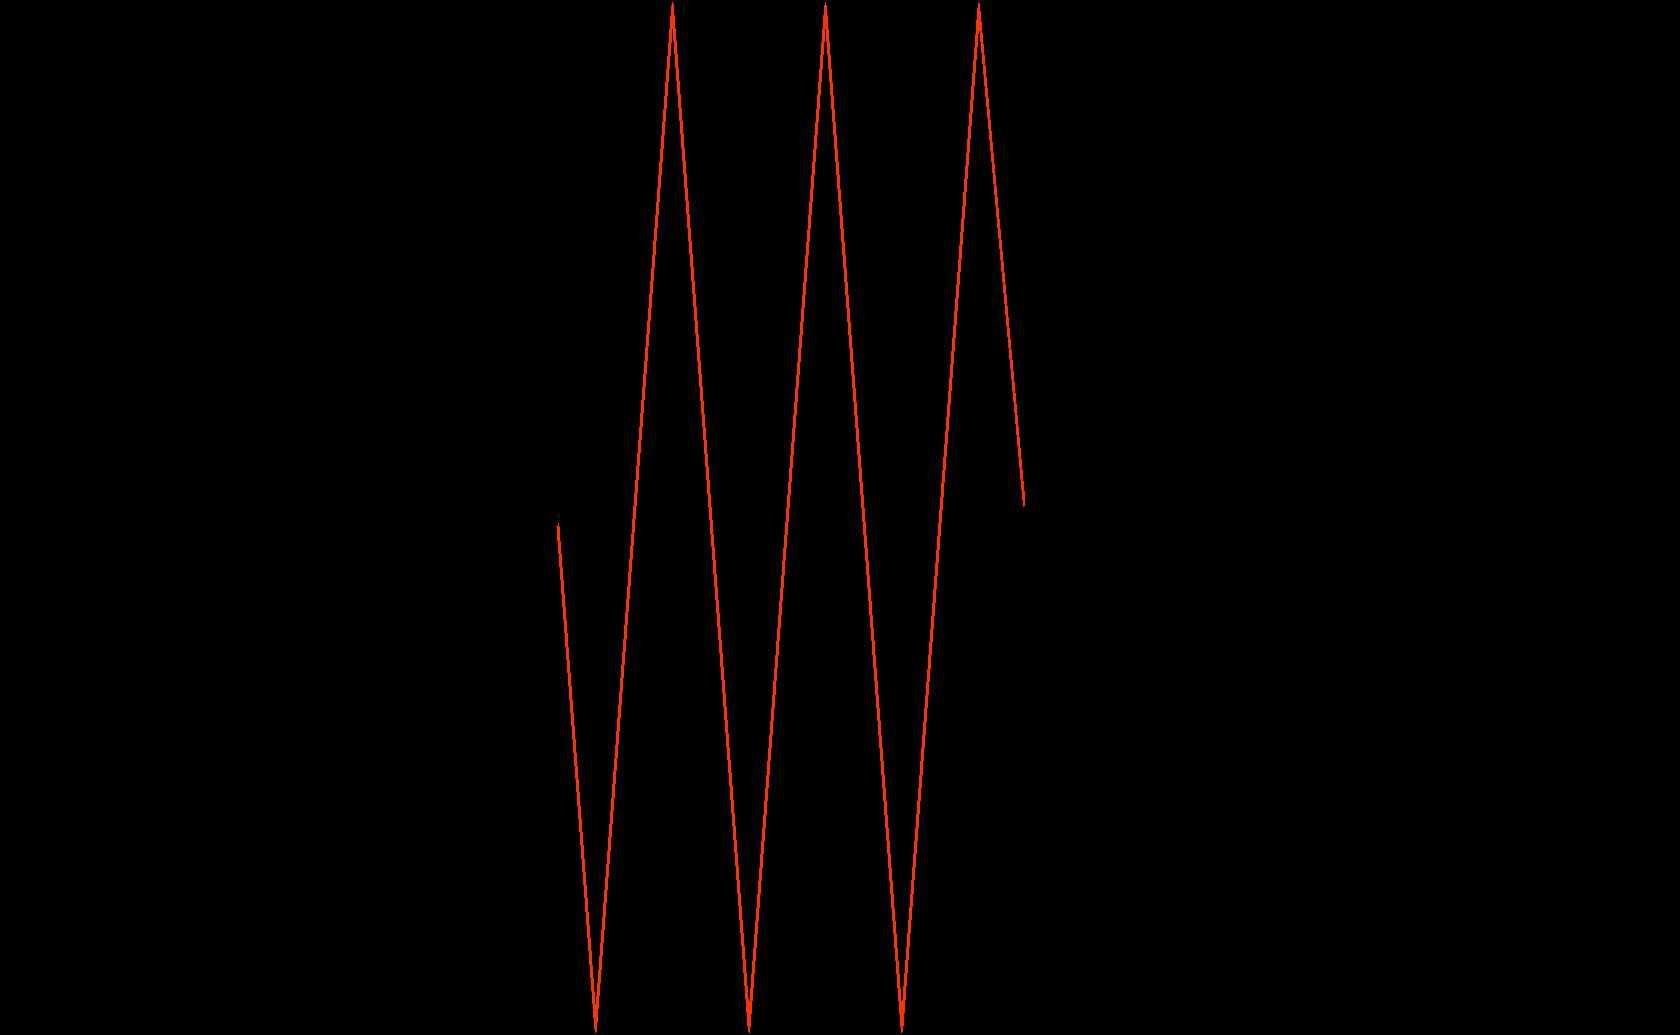
\includegraphics[width=1.742in,height=0.2794in]{Resister_symbol0}
\end{figure}for resistors, but they
often look more like this\begin{figure}[h!]
	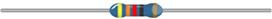
\includegraphics[width=2.2987in,height=0.179in]{PH4CAU11}
\end{figure}

Notice that this is important! We have found a way to relate our new
quantity that we want to measure, current, to a voltage. We know how to
measure a voltage! Our Ohm's law equation even tells us what extra part we
need to convert our voltmeter into a current measuring instrument. We will
need a resistor.

\subsubsection{Resistor Code}

Let's pause in our new instrument design for a moment and ask,
\textquotedblleft how would you know the resistance of a
resistor?\textquotedblright\ Our multimeters have a resistance measuring
setting, so you could measure the resistance directly using the meter. But
many commercially produced resistors come conveniently marked with a color
code that helps you identify their resistance. The basics of the color code
are given in the following figure\bigskip \begin{figure}[h!]
	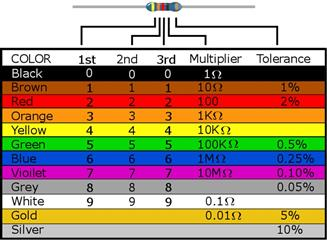
\includegraphics[width=3.2958in,height=2.4249in]{PH4CAU12}
\end{figure}

To use the code:

\begin{enumerate}
	\item Find the tolerance code band. This band is usually brown in our kit
	resistors and often is set off from the others a little more.
	
	\item Read the first color band from the side opposite the tolerance band.
	This will be the first digit of your resistance. I\ think the example
	resister on the chart has a yellow first color band, so the first digit of
	our resistance is $4.$
	
	\item Read the second color band. This will be the second digit of your
	resistance. I\ think the second band of our example resistor is orange, so
	the second digit would be a $3,$ making our resistance so far $43$
	
	\item Read the third color band. This will be the third digit of your
	resistance. I\ think the second band of our example resistor is red, so the
	second digit would be a $2,$ making our resistance so far $432$
	
	\item Read the forth color band. This is a multiplier. You multiply the
	first three digits by this amount. For our example resistance, I think the
	third band is black. Then we multiply $432$ by $1\unit{%
		%TCIMACRO{\U{3a9}}%
		%BeginExpansion
		\Omega%
		%EndExpansion
	}$ to get $432\unit{%
		%TCIMACRO{\U{3a9}}%
		%BeginExpansion
		\Omega%
		%EndExpansion
	}.$ This is our resistance.
	
	\item The tolerance band gives the uncertainty in this value. Our example
	resistor seems to have a brown tolerance band, which tells us our value is
	good to $\pm 1\%.$ For our example resistance, $1\%$ would be $0.01\times 432%
	\unit{%
		%TCIMACRO{\U{3a9}}%
		%BeginExpansion
		\Omega%
		%EndExpansion
	}=\allowbreak 4.\,\allowbreak 32\unit{%
		%TCIMACRO{\U{3a9}}%
		%BeginExpansion
		\Omega%
		%EndExpansion
	},$ so our resistance is $\left( 432\pm 4\unit{%
		%TCIMACRO{\U{3a9}}%
		%BeginExpansion
		\Omega%
		%EndExpansion
	}\right) .$
\end{enumerate}

We won't memorize the resistor code, but you should be able to find a
resistance using the code.

If you are in doubt about what color you see on a resistor, our multimeters
can measure resistance directly. \begin{figure}[h!]
	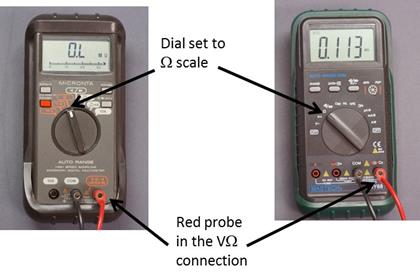
\includegraphics[width=3.5426in,height=2.3594in]{PH4CAU13}
\end{figure}Place the red probe in the
connector with a $\Omega $ marked on it and turn the dial to the $\Omega $
setting. Place the probes on either side of the resistance to be measured.
Be careful/ You are a resistor too. If you touch your hands to the probes
(common mistake while you try to hold the resistor on the probe ends) you
may measure your resistance instead of the resistor's! You have a resistance
of around half a megaohm. This is a general concern, every time you measure
resistance with a meter you need to take the circuit element (resistor,
light bulb, whatever) out of the circuit and measure it on it's own.
Otherwise, you might be measuring the resistance of the rest of the circuit.
Alligator clips are useful for this.

\subsubsection{Direction of current flow}

There is a historical oddity with current flow. That is that the current
direction is the direction positive charges would flow. This may seem
strange, since in good conductors electrons are doing the flowing and they
are negative! The electrons go the opposite way the current goes. \begin{figure}[h!]
	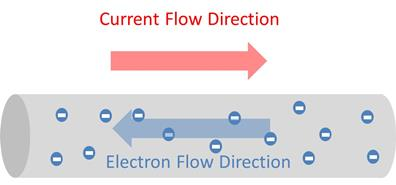
\includegraphics[width=3.3373in,height=1.5696in]{PH4CAU14}
\end{figure}%
The truth is that it is very hard to tell the difference between positive
charge flow and negative charge flow the other direction. In fact, only one
experiment that I know of shows that the charge carriers in metals are
electrons. And mathematically, the flow of electrons one direction is
equivalent to the flow of positive charges the other direction.\begin{figure}[h!]
	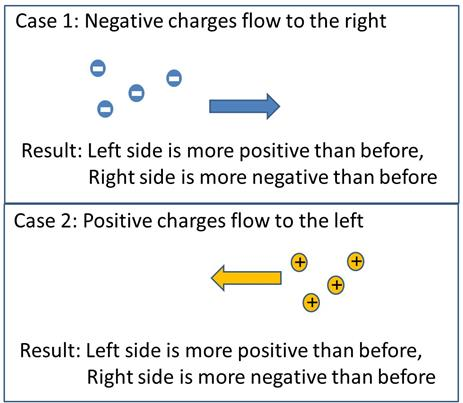
\includegraphics[width=%
	3.8994in,height=3.3961in]{PH4CAU15}
\end{figure}%
Worse yet, in biological things it \emph{is} positive ions that flow. So for
biology a positive charge carrier is just fine.

Ben Franklin chose the direction we now use. He had a 50\% chance of making
it easy for our electronics lab. But he got it backwards for us (but right
for biology--and how many electronic things did Ben Franklin have anyway?).
All this shows just how hard it is to deal with all these things we can't
see or touch that we study in PH 220.

And even more importantly, in semiconductors--special electronic devices in
all computers and in our Arduinos--it \emph{is} positive charge that flows.
In many electrochemical reactions \emph{both} positive and negative charges
flow. So Mr. Franklin was not really so very wrong. We will stick with the
convention that \textbf{the current direction is the direction that positive
	charges would flow regardless of the actual charge carrier motion. }If you
are like me, this will seem a little backwards, but we all get used to it.

But what makes the electrons or positive charges want to flow in the first
place? We know the answer to this from earlier in this lab reading. It is
potential energy. When we connect a metal wire to the terminals of a battery
we know that the charges in the metal wire ends will experience a difference
in potential energy. The potential energy difference will set up an electric
field inside the conductor. \begin{figure}[h!]
	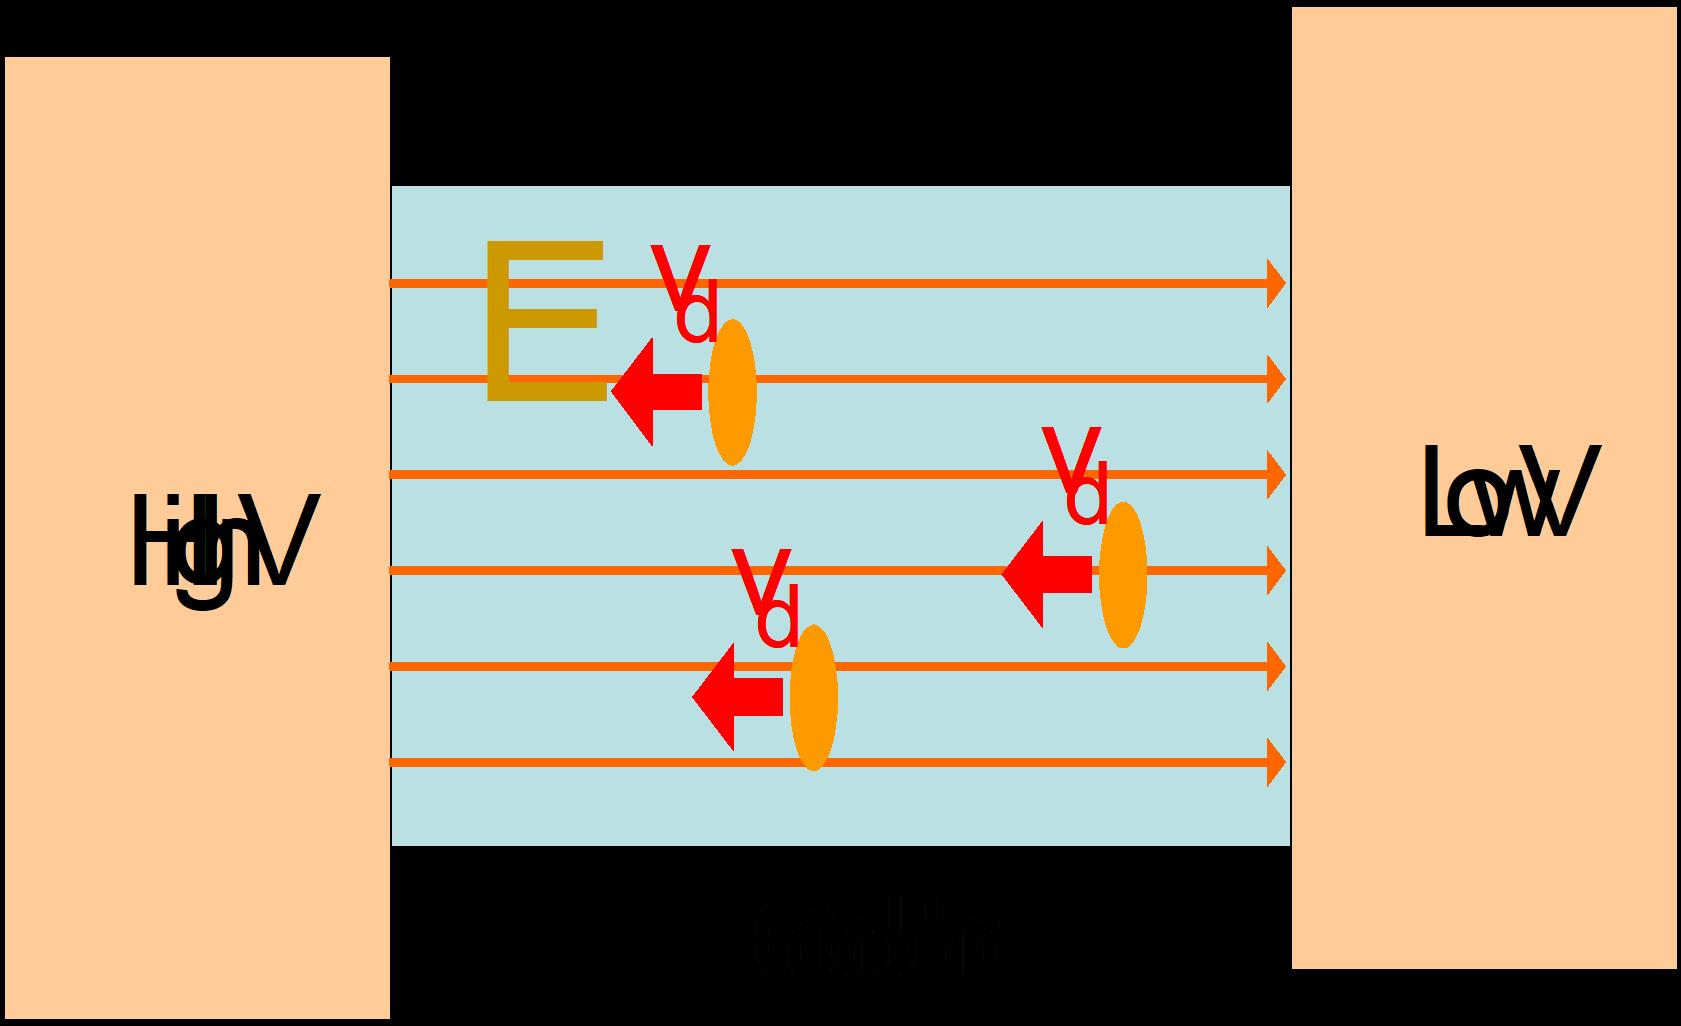
\includegraphics[width=4.2832in,height=1.0253in]{PH4CAU16}
\end{figure}

This field makes the free charges move! It causes a force on the little
electrons. We won't have to measure any fields in our lab today, but you
should know they are there. The important thing is to realize that voltages
produce currents. And the amount of current is proportional to the amount of
voltage. This is just Ohm's law! 
\begin{equation*}
\Delta V=IR
\end{equation*}%
The constant of proportionality is related to how much friction there is for
the charges in the wire.%
\begin{equation*}
I=\frac{1}{R}\Delta V
\end{equation*}%
It is just the resistance, $R$.\ 

\subsection{Knowing the Physics, Design the new instrument}

Now that we understand electrical current, we have some hope of figuring out
how to build an instrument to measure that electrical current. From what we
learned, consider adding in an additional small resistor in our circuit. If
we take a small resistance, one that is small compared to all the other
resistances in the circuit, and we put it in the circuit it will slow down
the current, but not by very much. If the resistance is small enough, we
won't even notice the change. Then if we measure the voltage across that
small resistor with a voltmeter, we could mathematically calculate how much
current we have. Notice that this instrument design has two parts. The first
is adding some new hardware to our voltmeter (a resistor) and the second is
adding in some calculation to get our voltmeter reading converted into
current. 
\begin{equation*}
I=\frac{1}{R}\Delta V
\end{equation*}

Let's give this additional small resistor a name. Let's call it the
\textquotedblleft shunt resistor.\textquotedblright\ 
\begin{equation*}
I=\frac{\Delta V_{meter}}{R_{shunt}}
\end{equation*}%
Today we will have to do the calculation part by hand. In future labs, we
would carefully plan for this calculation in our Arduino sketch code.

\begin{figure}[h!]
	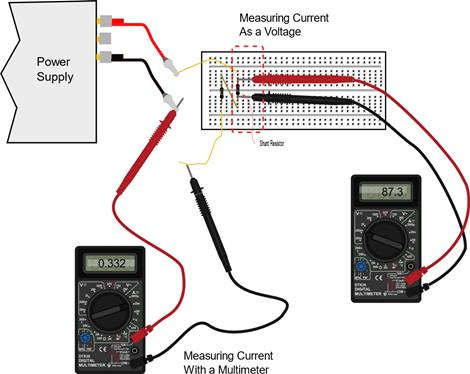
\includegraphics[width=4.9156in,height=3.9176in]{PH4CAU17}
\end{figure}

When we are done wiring our new instrument, we will have done something
really cool. We have turned our current measurement into a voltage
measurement. We measured something new in terms of a measurement we already
knew how to make. We will generally try to do this for any type of
measurement. That is because we are very good at measuring voltage, and not
so good at measuring other things electronically.

\subsection{Testing the new instrument}

We will need a way to test how good our new instrument works. And
fortunately we know our multimeters can also measure current. So we can
build our new instrument an compare it to the measurement made by a
multimeter. 
\begin{equation*}
\unit{A}=\frac{\unit{V}}{\unit{%
		%TCIMACRO{\U{3a9}}%
		%BeginExpansion
		\Omega%
		%EndExpansion
}}
\end{equation*}%
Recall that to use an ammeter (the new instrument we build, or the one in
our multimeter), you must break the electric circuit by disconnecting a
wire. Then you replace that wire with the ammeter. Notice that in the
diagram below that the bottom wire is now broken. \begin{figure}[h!]
	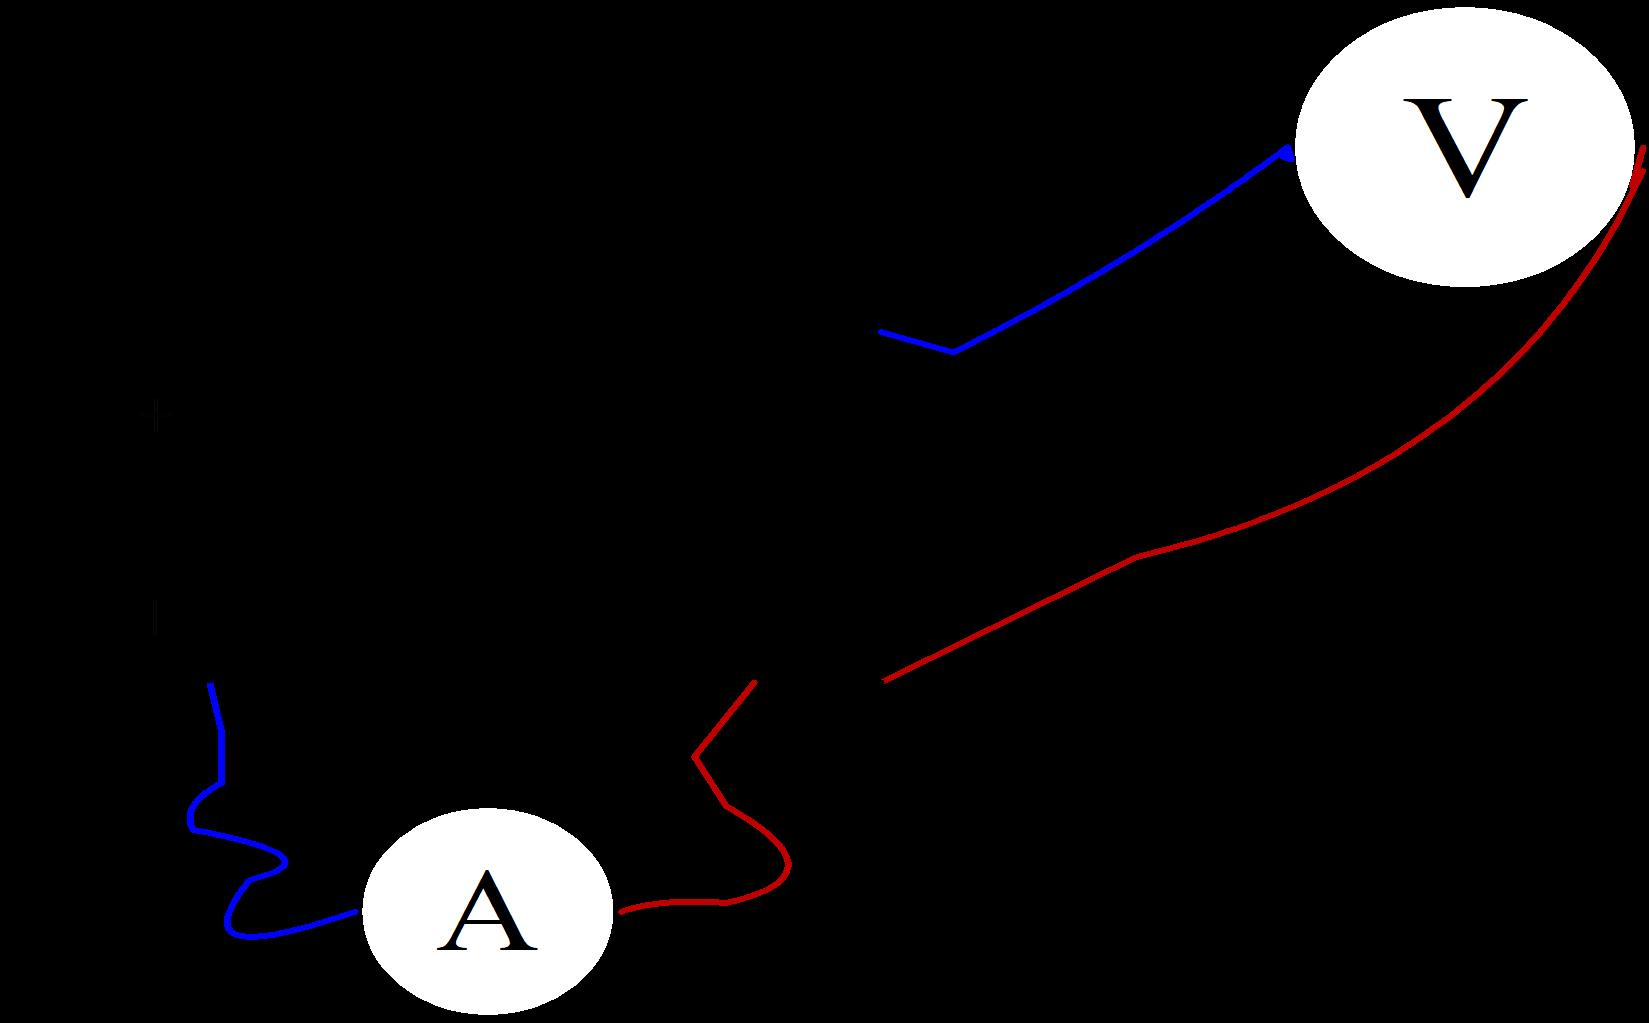
\includegraphics[width=1.9372in,height=%
	1.471in]{PH4CAU18}
\end{figure}Where a wire was, I have drawn an
ammeter. The current must flow through the ammeter for us to measure it.

\begin{figure}[h!]
	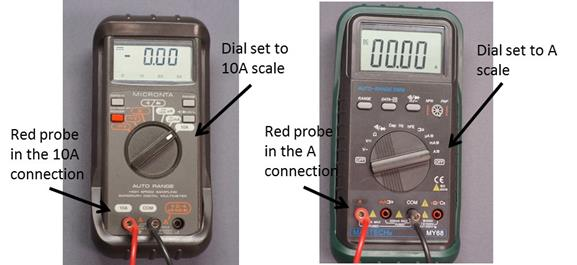
\includegraphics[width=4.858in,height=2.2423in]{PH4CAU19}
\end{figure} Remember, to use our multimeters
to measure current, we must turn the dial to the $10\unit{A}$ setting AND
move the red probe to the $10\unit{A}$ connector. Failure to do this may
result in the fuse blowing. Our meter does not warn you that it lost a fuse,
it just pays you back by giving really wrong answers. You should be careful
to connect it right, and be sure it is working (that someone else has not
blown the fuse before you). Since we have different kinds of multimeters, a
second is pictured to the right. For this type of meter, put the red lead in
the connector marked $A$ and turn the dial to the $A$ setting. If the
currents you are measuring are very small, you might have to switch settings
once again. Tiny currents can be measured by moving the dial to the $\unit{mA%
}$ setting AND changing the red probe to the $\unit{mA}$ connector.\begin{figure}[h!]
	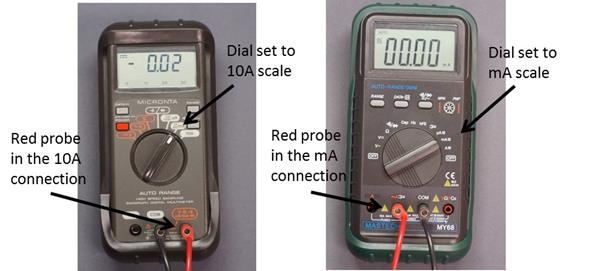
\includegraphics[width=4.9769in,height=2.2928in]{PH4CAU1A}
\end{figure}

Our multimeters really measure current in much the same way we are talking
about for our new Arduino ammeter. They have a series of shunt resistors
inside of them. When we choose a current measurement setting we are choosing
a shunt resistor to put in the circuit (inside the meter, but the meter is
in the circuit). Then the voltmeter will measure the voltage across that
resistor and use that voltage to calculate the current.

If we create the current meter ourselves, we have to know the resistance
that we used! That allows us to use the voltage meter to calculate the
current,%
\begin{equation*}
I=\frac{\Delta V_{meter}}{R_{shunt}}
\end{equation*}%
but our multimeters are programed to know their own shunt resistances and to
do this calculation for us.

If you have time (and some won't) in today's lab, we will build the new
Arduino instrument to measure current , and we will test it with a
multimeter set in ammeter mode. We will put both in the circuit at the same
time (see figure \ref{New Instrument and Test}) so we get readings from
both. Then we can compare and see how well our new instrument works!

\section{Calculating uncertainty, a review}

That is all the new material for today's lab. But I wanted to remind you of
something you already know.

Back in PH150 you should have gotten a good deal of experience in making
measurements. We will be going back to experimentation soon, and we will
need to remember what we learned in PH150 to take the measurements so that
we can interpret our experimental results. You will remember that every
measurement has an uncertainty. We have to estimate that uncertainty. It
turns out that our voltage measurement schemes will introduce a new source
of uncertainty! And we will have to include this in our uncertainty
calculations. We will take that on next lab, but in this lab let's review
how to calculate uncertainties.

This is a \textquotedblleft review.\textquotedblright\ How much of a
\textquotedblleft review\textquotedblright\ it is may depend on where and
when you took PH150 or its equivalent. If you are a chemist, you will note
that our treatment of uncertainty goes beyond what you learned in
Quantitative Analysis. Let's start by reviewing what a derivative is.

For our purposes, a derivative is a slope of a line. You should recognize
the equation of a straight line as%
\begin{equation*}
y=mx+b
\end{equation*}%
The slope $m$ can be written as 
\begin{equation*}
m=\frac{dy}{dx}
\end{equation*}%
This is nothing magic (or new). It is just a strange way to write $m.$ With
the slope written this way, the equation of the line could be written as 
\begin{equation*}
y=\frac{dy}{dx}x+b
\end{equation*}%
But why $dy/dx$? Think of how we find a slope of a line. Back in junior high
school we called the slope the \textquotedblleft rise over
run.\textquotedblright\ That is, the change in $y$-value divided by the
change in the $x$-value.%
\begin{equation*}
m=\frac{y_{2}-y_{1}}{x_{2}-x_{1}}
\end{equation*}%
In physics, we write the change in a variable using the greek letter delta, $%
\Delta .$ So we could write the slope as%
\begin{equation*}
m=\frac{y_{2}-y_{1}}{x_{2}-x_{1}}=\frac{\Delta y}{\Delta x}
\end{equation*}%
\ Just to jog your memory, let me write out $\Delta y$%
\begin{equation*}
\Delta y=y_{2}-y_{1}
\end{equation*}%
and $\Delta x.$ 
\begin{equation*}
\Delta x=x_{2}-x_{1}
\end{equation*}%
So our straight line equation should be written 
\begin{equation*}
y=\frac{\Delta y}{\Delta x}x+b
\end{equation*}%
but if we take $\Delta x$ to be very, very small it is customary to write
the $\Delta x$ as just $dx$ (I guess a \textquotedblleft $d$%
\textquotedblright\ is smaller than a \textquotedblleft $\Delta $%
\textquotedblright ). If this is not familiar from Math 112, is should be by
now from PH121.

In PH121 you learned that the velocity is the slope of the plot of $x$ vs. $%
t,$ for example, 
\begin{equation*}
y=\frac{1}{2}\frac{\unit{m}}{\unit{s}}t+1\unit{m}
\end{equation*}%
is an equation giving the $y$ position of an object as a function of time.
Note that it is a straight line on a $y$ vs. $t$ plot. \begin{figure}[h!]
	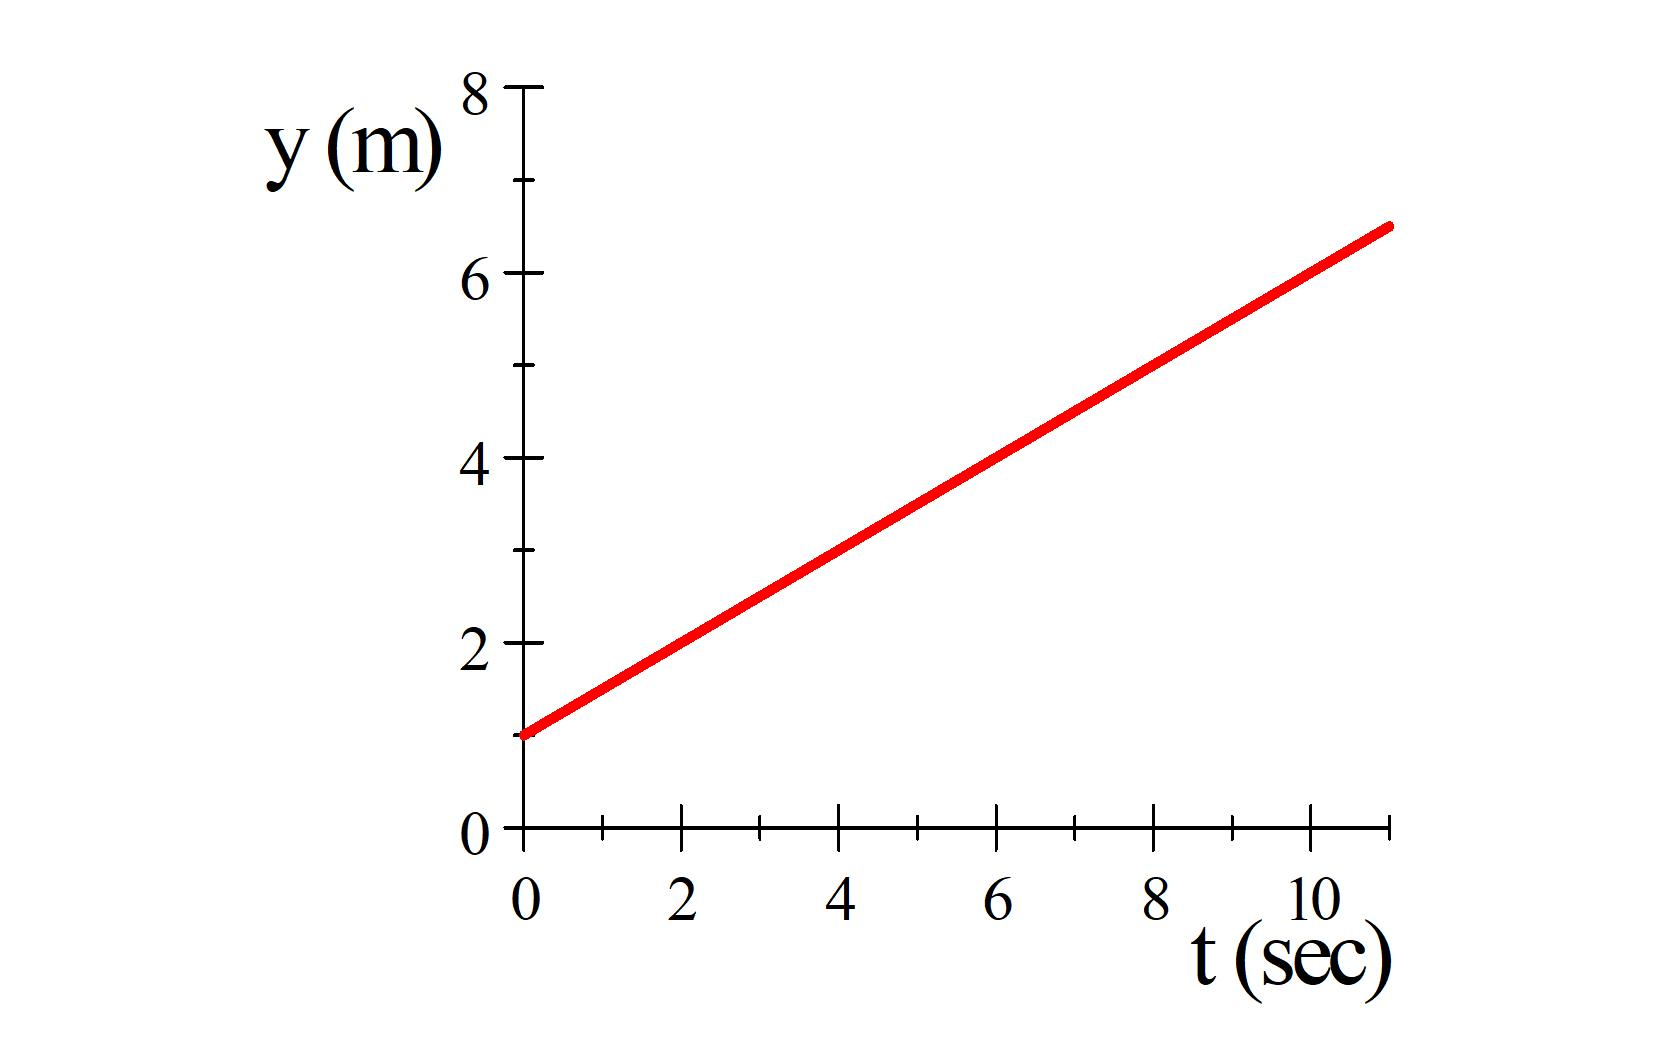
\includegraphics[width=%
	3.4999in,height=1.868in]{PH4CAU1B}
\end{figure}The slope of the line is 
\begin{equation*}
\frac{dy}{dt}=\frac{1\unit{m}}{2\unit{s}}
\end{equation*}%
We can verify that this works by looking at the plot and noting that for
every two units of time, we go up one position unit. The slope is $1/2\frac{%
	\unit{m}}{\unit{s}}.$

But not all curves are straight lines. What do we do with curves that, well,
curve?

One idea is that we could split up the curve into little line segments, each
with its own slope. We can think of $dy/dt$ as an instantaneous slope, a
slope of one of the tiny line segments that make up our curve. This is the
sort of speed measurement that your speedometer gives. The speed might be
different a short time later. But right now the speed is, say, $0.5\unit{m}/%
\unit{s}.$

\begin{figure}[h!]
	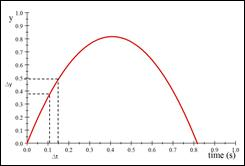
\includegraphics[width=3.4385in,height=2.3307in]{PH4CAU1C}
\end{figure}Really, in defining an
instantaneous slope we have assumed that the slope near our point on the
curve is essentially a straight line if $\Delta t$ is small enough.

We can use this idea to interpret our error calculations. Suppose I\ throw a
ball in the air with a initial speed of $4\unit{m}/\unit{s}$ straight up
starting from $y_{o}=0$. From PH121 you have learned that the equation for
predicting how high the ball will go is 
\begin{equation*}
y=y_{o}+v_{o}t+\frac{1}{2}at^{2}
\end{equation*}%
It says that starting at $y_{o}$ the ball will go higher depending on the
initial velocity, $v_{o},$ and the acceleration, $a.$ That makes sense.

At a time, $t,$ the ball should be at 
\begin{equation*}
y=0+4\frac{\unit{m}}{\unit{s}}t-\frac{1}{2}\left( 9.8\frac{\unit{m}}{\unit{s}%
	^{2}}\right) t^{2}
\end{equation*}%
where $a=-9.8\frac{\unit{m}}{\unit{s}^{2}}$ is the acceleration due to
gravity. So, knowing this, I could predict how high the ball would go if I\
pick a particular time, say, $0.15\unit{s}.$ The result should be%
\begin{eqnarray*}
	y &=&0+4\frac{\unit{m}}{\unit{s}}\left( 0.15\unit{s}\right) -\frac{1}{2}%
	\left( 9.8\frac{\unit{m}}{\unit{s}^{2}}\right) \left( 0.15\unit{s}\right)
	^{2} \\
	&=&0.489\,75\unit{m}
\end{eqnarray*}%
This is shown in the next figure with a black line. Solving the equation for 
$y$ is equivalent to drawing a line up to the curve, then from our spot on
the curve over to the $y$-axis to find the position.\begin{figure}[h!]
	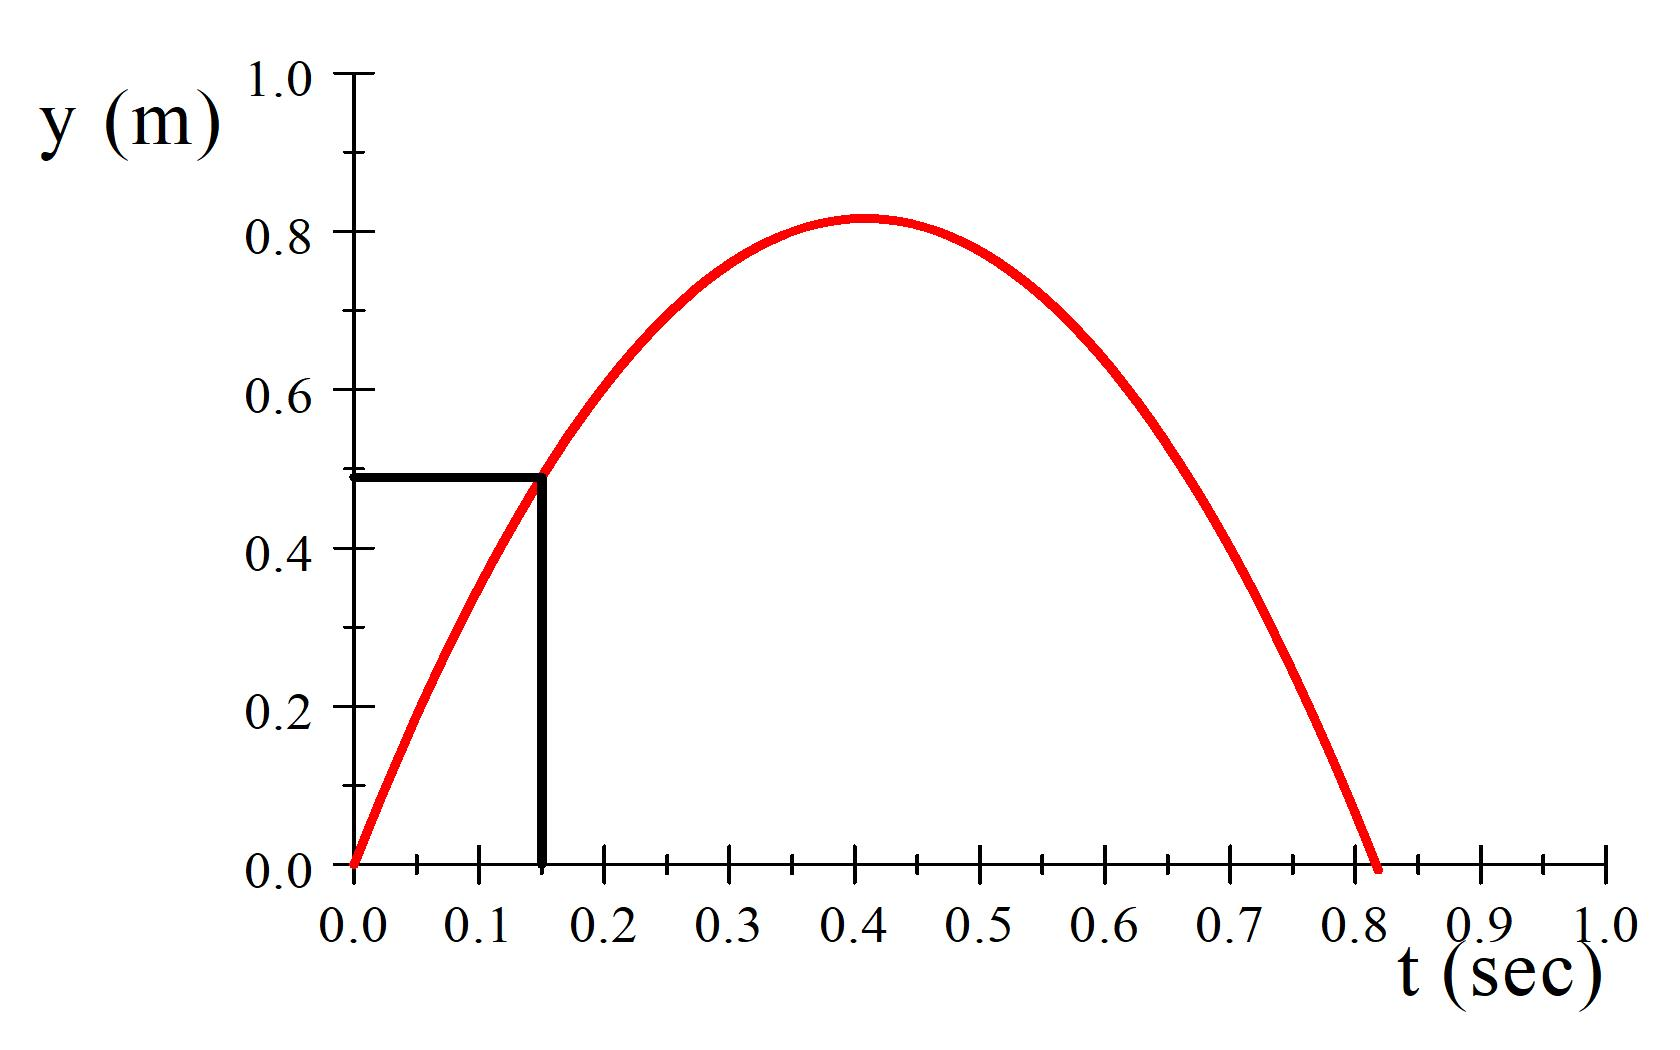
\includegraphics[width=3.3434in,height=%
	2.2295in]{PH4CAU1D}
\end{figure}

For our case, we plot a line upward from $0.15\unit{s}$ to the curve, and
then plot a horizontal line from the intersection to the $y$-axis. We can
see that we get $4.9\unit{m}.$ Suppose I try to verify this by taking a
picture of the ball in flight at $0.015\unit{s},$ but my stop watch is only
good to $\pm 0.005$ seconds. I try to take the picture when the watch is at $%
0.015\unit{s},$ but I might have taken the picture at $0.01\unit{s}$ or at $%
0.02\unit{s}$ or anywhere in between. My time has some uncertainty. What
does the uncertainty in my stop watch time mean for the uncertainty in my $y$
value?

We can get a good approximation by graphically drawing vertical lines up
from $t_{\min }$ and $t_{\max }$ to the curve, and then extending horizontal
lines from the intersections to the $y$-axis. This gives us a $y_{\min }$
and $y_{\max }.$ Our actual height could be anywhere in between these. This
is a way to view our uncertainty in $y.$\begin{figure}[h!]
	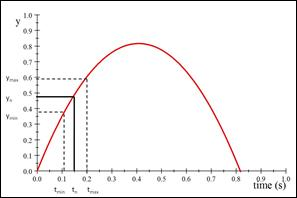
\includegraphics[width=4.1658in,height=2.7769in]{PH4CAU1E}
\end{figure}

We can use this idea to find a general way to calculate uncertainties. We
could define $\Delta t=t_{\max }-t_{\min }$. If our $\Delta t$ is small
enough (so we can write it just $dt$), the curve is essentially a straight
line in the region between $t_{\min }$ and $t_{\max }.$ So if we knew the
slope of that line (the derivative $dy/dt$) we could easily figure out the $%
y_{\max }$ and $y_{\min }$ points to get our uncertainty range, at least if
we stay near our $t_{n}$ part of the curve. Recall that our uncertainty in $%
y $ is about%
\begin{equation*}
\delta y=\frac{y_{\max }-y_{\min }}{2}=\frac{\Delta y}{2}
\end{equation*}%
Remembering that 
\begin{equation*}
y=\frac{dy}{dt}t+b
\end{equation*}%
then 
\begin{eqnarray*}
	\Delta y &=&y_{\max }-y_{\min } \\
	&=&\frac{dy}{dt}t_{\max }+b-\frac{dy}{dt}t_{\min }-b \\
	&=&\frac{dy}{dt}\Delta t
\end{eqnarray*}%
From PH150, you will recognize this as almost the uncertainty in a function
of one variable! But even if you don't recognize it, we can show that this
is true using our definition of $\delta y$ above. The quantity $\Delta t$ is 
\begin{equation*}
\Delta t=t_{\max }-t_{\min }
\end{equation*}%
so our uncertainty in $t$ would be 
\begin{equation*}
\delta t=\frac{t_{\max }-t_{\min }}{2}=\frac{\Delta t}{2}
\end{equation*}%
then 
\begin{eqnarray*}
	\delta y &=&\frac{y_{\max }-y_{\min }}{2} \\
	&=&\frac{1}{2}\frac{dy}{dt}\Delta t \\
	&=&\frac{dy}{dt}\frac{\Delta t}{2} \\
	&=&\frac{dy}{dt}\delta t
\end{eqnarray*}%
so%
\begin{equation*}
\delta y=\frac{dy}{dt}\delta t
\end{equation*}%
So our uncertainty in $y$ is just the slope at our point on the curve
multiplied by our uncertainty in $t.$

But what if we have more than one variable? Say, we have a function $y(x,z),$
we essentially have a two dimensional slope. Think of a hill, you can go
down a hill in more than one direction. So we need slope parts for each
direction we can go.

\begin{figure}[h!]
	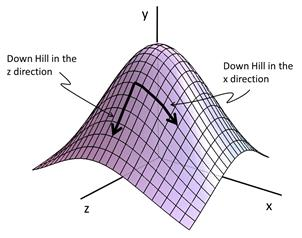
\includegraphics[width=2.5495in,height=2.0133in]{PH4CAU1F}
\end{figure}%
\begin{equation*}
\Delta y=\frac{dy}{dx}x\hat{\imath}+\frac{dy}{dz}z\hat{k}
\end{equation*}%
But there is a fix we need to make to this equation that you won't learn for
several math classes to come. We want to have a slope in the $x$ and $z$
direction, but we want the slopes to be independent (if you have already
taken PH121, think of two dimensional motion problems, we split the problem
into components). The notation for this is%
\begin{equation*}
\Delta y_{x}=\frac{\partial y}{\partial x}x
\end{equation*}%
\begin{equation*}
\Delta y_{z}=\frac{\partial y}{\partial z}z
\end{equation*}%
where 
\begin{equation*}
\frac{\partial y}{\partial x}
\end{equation*}%
means the component of the slope just in the $x$ direction. We take a
derivative of the function $y,$ but assume only $x$ is a variable (treat $z$
and all $z$ terms with no $x^{\prime }s$ as constants). This lets us
separate the $x$ and $z$ parts. A special, one variable derivative like $%
\partial y/\partial x$ is called a \emph{partial derivative} because you
only take one dimension of the derivative at a time. So, if we wish to find
the error in some general function $z\left( x,y\right) $ the error is given
by 
\begin{equation*}
\delta y=\sqrt{\left( \frac{\partial y}{\partial x}\right) ^{2}\delta
	x^{2}+\left( \frac{\partial y}{\partial z}\right) ^{2}\delta z^{2}}
\end{equation*}%
This looks a lot like our slope equation. What we are doing is to assuming
the function $y\left( x,z\right) $ is flat in a small region around the
point we are studying. then the function has a slope $\partial y/\partial x$
in the $x$-direction, and $\partial y/\partial z$ in the $y$-direction. Each
term like 
\begin{equation*}
\left( \frac{\partial y}{\partial x}\right) \delta x
\end{equation*}%
gives how far off we could be in that direction (the $x$-direction in this
case). Remember that we have assumed that $y\left( x,z\right) $ is
essentially flat near our point of interest. The square root may be
something of a mystery, but remember what you have learned about adding
vectors in PH121. We add components of a vector to find the magnitude like
this 
\begin{equation*}
V=\sqrt{V_{x}^{2}+V_{y}^{2}}
\end{equation*}%
This comes from the Pythagorean theorem. The $x$ and $y$ parts of the vector
form two sides of a triangle. We want the remaining side. So we use the
Pythagorean theorem to find the length of the remaining side.

We are doing the same for our small uncertainty lengths. We are just adding
the $x$ and the $y$ components of the error. We could write our error
formula for the general case of a function $f$, that depends on $N$
different variables. 
\begin{equation*}
\delta f=\sqrt{\sum_{i=1}^{N}\left( \frac{\partial f}{\partial x_{i}}\right)
	^{2}\delta x_{i}^{2}}
\end{equation*}%
We will use this formula a lot, so make sure you understand what it means
(ask your instructor for help if it is not clear).

\subsection{How do we find the slope?}

But now we have an equation in terms of slope written as $\partial
y/\partial x$ or $\partial y/\partial z$, but how would we ever find these
slopes? Your calculus class has or will teach you how to take a derivative.
They might not have yet taught you how to take this type of derivative. The
symbol $\partial $ means that our derivatives are \textquotedblleft
partial\textquotedblright\ derivatives. This means that we assume all the
variables other than the one that shows up in the derivative symbol are
constants for our derivative.

Let's take an example. What is the slope of the function $y=5zx^{3}?$ if we
calculate the slope only going in the $x$-direction (that is, if we take a
partial derivative with respect to $x$) we get

\begin{equation*}
\frac{\partial }{\partial x}\left( 5zx^{3}\right) =5z\left( 3\right)
x^{3-1}=15zx^{2}
\end{equation*}%
notice that we treated $z$ as a constant! That is what we mean when we user
the symbol $\partial $ and when we say \textquotedblleft partial
derivative.\textquotedblright\ Let's try another. How about finding the
slope of $f=7yx^{2}-2x+z$ with respect to the $x$-direction.

\begin{equation*}
\frac{\partial }{\partial x}\left( 7yx^{2}-2x+z\right) =7y\left( 2\right)
x^{1}-2(1)x^{0}+z\left( 0\right)
\end{equation*}%
The last term illustrates that the slope of a constant is zero, and as we go
just in the $x$-direction, $z$ is constant. That makes sense. So the change
in $f$ just due to the last term $(z)$ should be zero. We also remember $%
x^{0}=1.$ So we are left with 
\begin{equation*}
\frac{\partial }{\partial x}\left( 7yx^{2}-2x+z\right) =14yx-2
\end{equation*}%
We could also find 
\begin{equation*}
\frac{\partial }{\partial y}\left( 7yx^{2}-2x+z\right) =7x^{2}
\end{equation*}%
and%
\begin{equation*}
\frac{\partial }{\partial z}\left( 7yx^{2}-2x+z\right) =1
\end{equation*}

In our equation for calculating uncertainties, we want to find the
uncertainty in each dimension (for each variable) and to add these
uncertainties like components of vectors, so this partial derivative is just
what we want, the slope of our function in just one direction.

\subsubsection{Tie to statistics}

Back in PH150 you should have learned that for experiments where we repeat
the same experiment over and over again, our outcome can be given by the
mean value an our uncertainty can be given by the standard deviation. We
need to tie our statistical ideas into what we have learned about error
propagation. Lets go back to our function $f\left( x,z\right) $ the error is
given by 
\begin{equation*}
\delta f=\sqrt{\left( \frac{\partial f}{\partial x}\right) ^{2}\delta
	x^{2}+\left( \frac{\partial f}{\partial z}\right) ^{2}\delta z^{2}}
\end{equation*}%
but now we know we could express this in terms of standard deviations
(provided you don't need to ensure every bit of your data are within your
uncertainty range). We can write our uncertainties as 
\begin{equation*}
\sigma _{f}=\sqrt{\left( \frac{\partial f}{\partial x}\right) ^{2}\sigma
	_{x}^{2}+\left( \frac{\partial f}{\partial z}\right) ^{2}\sigma _{z}^{2}}
\end{equation*}%
So one way to get an estimate of uncertainty like $\delta x$ or $\delta z$
above is to make many measurements, and use the standard deviation $\sigma
_{x}$ as an estimate for $\delta x$ and $\sigma _{z}$ for $\delta z.$ This
is usually not too far off (we will refine this analysis in PH336 for those
lucky enough to take the course).

We can use connection between $\delta x$ and $\sigma _{x}$ to show that the
standard deviation of the mean (the best estimate of our uncertainty) is
given by

\begin{equation*}
\sigma _{\bar{x}}=\frac{\sigma _{x}}{\sqrt{N}}
\end{equation*}%
(a result you should have learned back in PH150). Think of calculating a
mean value%
\begin{equation*}
\bar{x}=\frac{x_{1}+x_{2}+\cdots x_{N}}{N}
\end{equation*}%
We can find the uncertainty in this function $\sigma _{\bar{x}}$%
\begin{equation*}
\sigma _{\bar{x}}=\sqrt{\left( \frac{\partial \bar{x}}{\partial x_{1}}%
	\right) ^{2}\sigma _{x_{1}}^{2}+\left( \frac{\partial \bar{x}}{\partial x_{2}%
	}\right) ^{2}\sigma _{x_{2}}^{2}+\cdots +\left( \frac{\partial \bar{x}}{%
		\partial x_{N}}\right) ^{2}\sigma _{x_{N}}^{2}}
\end{equation*}%
You see we just take the partial derivative of our function $\bar{x}$ with
respect to each of the variables $x_{i}$ and multiply by the uncertainty in
that variable written now as a standard deviation $\sigma _{i}.$

For this special case, all of the $x_{i}$ are the same (we are measuring the
same value over and over in taking an average) and all of the $\sigma _{i}$
are the same so we just have%
\begin{equation*}
\sigma _{\bar{x}}=\sqrt{N\left( \frac{\partial \bar{x}}{\partial x_{1}}%
	\right) ^{2}\sigma _{x_{1}}^{2}}
\end{equation*}%
and we can take the derivative using our rule. Only $x_{1}$ is a variable,
so we can write the average $\bar{x}$ as 
\begin{equation*}
\bar{x}=\frac{x_{1}}{N}+\frac{x_{2}+\cdots x_{N}}{N}
\end{equation*}%
This is a polynomial! The first term is $\frac{1}{N}x_{1}$ and the whole
second term is a constant if we take a partial derivative with respect to $%
x_{1}$. The derivative is 
\begin{eqnarray*}
	\frac{\partial \bar{x}}{\partial x_{1}} &=&\frac{\partial }{\partial x_{1}}%
	\left( \frac{x_{1}}{N}+\frac{x_{2}+\cdots x_{N}}{N}\right) \\
	&=&\frac{1}{N}x_{1}^{0}+0 \\
	&=&\frac{1}{N}
\end{eqnarray*}%
so our statistical error function is just 
\begin{eqnarray*}
	\sigma _{\bar{x}} &=&\sqrt{N\left( \frac{1}{N}\right) ^{2}\sigma _{x_{1}}^{2}%
	} \\
	&=&\sqrt{\frac{\sigma _{x_{1}}^{2}}{N}} \\
	&=&\frac{\sigma _{x_{1}}}{\sqrt{N}}
\end{eqnarray*}%
or, since all the $\sigma _{x_{i}}$ are the same, we can just write this as%
\begin{equation*}
\sigma _{\bar{x}}=\frac{\sigma _{x}}{\sqrt{N}}
\end{equation*}

Notice that in this example we had many $x_{i}$ and that to find the
uncertainty we just extended our equation from two variables%
\begin{equation*}
\sigma _{f}=\sqrt{\left( \frac{\partial f}{\partial x}\right) ^{2}\sigma
	_{x}^{2}+\left( \frac{\partial f}{\partial z}\right) ^{2}\sigma _{z}^{2}}
\end{equation*}%
to $N$ variables%
\begin{equation*}
\sigma _{f}=\sqrt{\sum_{i=1}^{N}\left( \frac{\partial f}{\partial x_{i}}%
	\right) ^{2}\sigma _{i}^{2}}
\end{equation*}

In this special case, we were trying to show a special result, but we can do
this for any function with any number of variables. If your function is
complicated, you just need to take more partial derivative terms under the
square root.



%\subsection{Build a new instrument from an old instrument}
%
%\begin{enumerate}
%\item IF\ THERE\ IS\ TIME, choose a resistor in the $20\unit{k%
%%TCIMACRO{\U{3a9}}%
%%BeginExpansion
%\Omega%
%%EndExpansion
%}$ range (say, from about $10\unit{k%
%%TCIMACRO{\U{3a9}}%
%%BeginExpansion
%\Omega%
%%EndExpansion
%}$ to about $30\unit{k%
%%TCIMACRO{\U{3a9}}%
%%BeginExpansion
%\Omega%
%%EndExpansion
%}$). Choose a shunt resistor in the $200\unit{%
%%TCIMACRO{\U{3a9}}%
%%BeginExpansion
%\Omega%
%%EndExpansion
%}$ range. Then set up the circuit to measure a current. \begin{figure}[h!]
%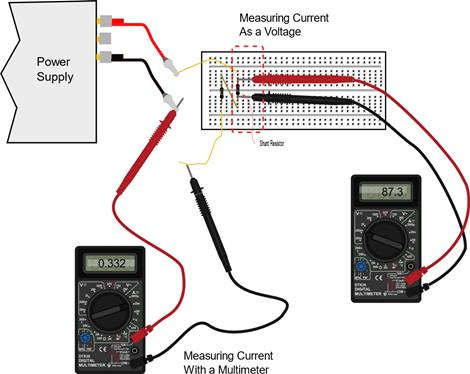
\includegraphics[width=%
%3.8744in,height=3.0874in]{PH4CAU1H}
%\end{figure}%
%Use an additional multimeter set to measure current to check our
%voltage-current measurement. Calculate a percent difference to see how well
%this worked.
%\end{enumerate}
%
%
%
%
%first, then before you connect the Arduino have group member check your
%wiring, then check the wiring with a stand-alone meter (that is why we
%learned to use them last week). Also remember, more than $5\unit{V}$ will
%damage the Arduino. So only put in voltages in the range $0\unit{V}$ to $5%
%\unit{V}.$
%
%We need one wire attached to the pin marked A0. We need another wire
%attached to one of our Arduino ground pins marked GND. And we connect the
%first wire to the positive output of our signal source (say, our power
%supply) and the GND wire to our negative output of our signal source (say
%the negative or ground connection on our power supply). That is all there is
%to it!
